\documentclass[tikz,border=6pt]{standalone}
\usepackage{amsmath}
\usetikzlibrary{arrows.meta,positioning,fit,decorations.pathreplacing}

\begin{document}
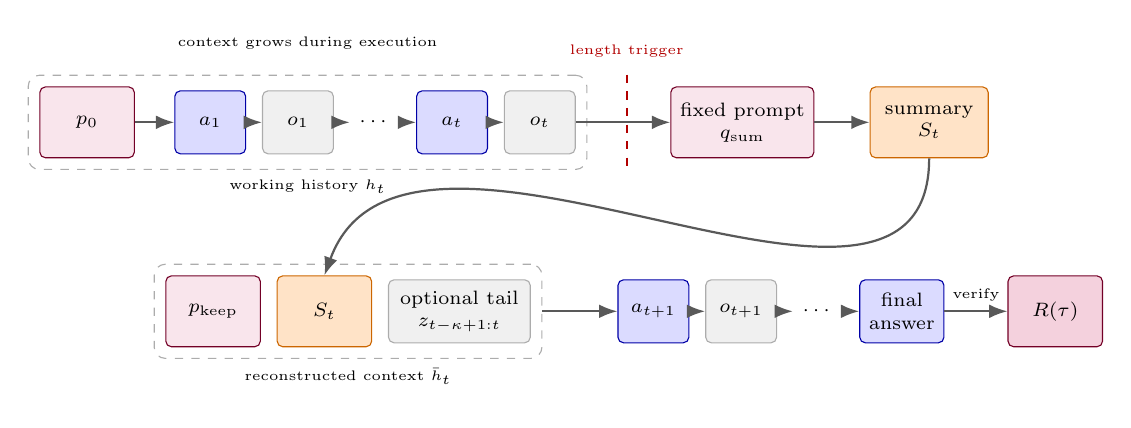
\begin{tikzpicture}[
  font=\scriptsize,
  >=Latex,
  flow/.style={->, thick, draw=gray!70!black},
  action/.style={
    rounded corners=2pt,
    draw=blue!65!black,
    fill=blue!14,
    minimum width=9mm,
    minimum height=8mm,
    align=center
  },
  observation/.style={
    rounded corners=2pt,
    draw=gray!65,
    fill=gray!12,
    minimum width=9mm,
    minimum height=8mm,
    align=center
  },
  summary/.style={
    rounded corners=2pt,
    draw=orange!80!black,
    fill=orange!22,
    minimum width=12mm,
    minimum height=9mm,
    align=center
  },
  fixed/.style={
    rounded corners=2pt,
    draw=purple!60!black,
    fill=purple!10,
    minimum width=12mm,
    minimum height=9mm,
    align=center
  },
  context/.style={
    rounded corners=4pt,
    draw=gray!65,
    dashed,
    inner sep=4pt
  },
  note/.style={align=center, font=\tiny}
]

% Growing context before compaction.
\node[fixed] (p0) at (0.4,2.65) {$p_0$};
\node[action, right=5mm of p0] (a1) {$a_1$};
\node[observation, right=2mm of a1] (o1) {$o_1$};
\node[right=2mm of o1] (dots1) {$\cdots$};
\node[action, right=2mm of dots1] (at) {$a_t$};
\node[observation, right=2mm of at] (ot) {$o_t$};
\node[context, fit=(p0)(ot), label={[note]below:working history $h_t$}] (history) {};
\node[note, above=2mm of history] {context grows during execution};

\draw[flow] (p0) -- (a1);
\draw[flow] (a1) -- (o1);
\draw[flow] (o1) -- (dots1);
\draw[flow] (dots1) -- (at);
\draw[flow] (at) -- (ot);

% Forced trigger and policy-generated summary.
\draw[red!70!black, dashed, thick]
  ([xshift=5mm]history.north east) -- ([xshift=5mm]history.south east);
\node[note, text=red!70!black, align=center]
  at ([xshift=5mm,yshift=3mm]history.north east)
  {length trigger};

\node[fixed, right=12mm of ot, minimum width=15mm] (qsum)
  {fixed prompt\\$q_{\mathrm{sum}}$};
\node[summary, right=7mm of qsum, minimum width=15mm] (summary)
  {summary\\$S_t$};
\draw[flow] (ot) -- (qsum);
\draw[flow] (qsum) -- (summary);

% Reconstructed context and continuation.
\node[fixed] (pkeep) at (2.0,0.25) {$p_{\mathrm{keep}}$};
\node[summary, right=2mm of pkeep] (summarycopy) {$S_t$};
\node[observation, right=2mm of summarycopy, minimum width=18mm] (tail)
  {optional tail\\$z_{t-\kappa+1:t}$};
\node[context, fit=(pkeep)(tail),
  label={[note]below:reconstructed context $\bar h_t$}] (reconstructed) {};

\node[action, right=11mm of tail] (anext) {$a_{t+1}$};
\node[observation, right=2mm of anext] (onext) {$o_{t+1}$};
\node[right=2mm of onext] (dots2) {$\cdots$};
\node[action, right=2mm of dots2] (afinal) {final\\answer};
\node[fixed, right=8mm of afinal, fill=purple!18] (reward) {$R(\tau)$};

\draw[flow] (summary.south) to[out=-90,in=70] (summarycopy.north);
\draw[flow] (reconstructed.east) -- (anext);
\draw[flow] (anext) -- (onext);
\draw[flow] (onext) -- (dots2);
\draw[flow] (dots2) -- (afinal);
\draw[flow] (afinal) -- node[above, note] {verify} (reward);

\end{tikzpicture}
\end{document}
